\documentclass[12pt, a4paper]{article}

% ============================================================
%  ENCODING & NGÔN NGỮ TIẾNG VIỆT
% ============================================================
\usepackage[utf8]{inputenc}
\usepackage[T5]{fontenc}
\usepackage[vietnamese]{babel}

% ============================================================
%  FONT — Times New Roman 13pt
% ============================================================
\usepackage{mathptmx}              % Times New Roman cho text và math
\usepackage{microtype}             % Cải thiện typography
\AtBeginDocument{\fontsize{13pt}{15.6pt}\selectfont}

% ============================================================
%  TRANG & LAYOUT
% ============================================================
\usepackage[
  a4paper,
  top=2.5cm, bottom=2.5cm,
  left=3cm,  right=2.5cm,
  headheight=14pt
]{geometry}
\usepackage{setspace}
\onehalfspacing               % Giãn dòng 1.5

% ============================================================
%  HEADER & FOOTER
% ============================================================
\usepackage{fancyhdr}
\pagestyle{fancy}
\fancyhf{}
\fancyhead[L]{\small\textit{Báo cáo Machine Learning}}
\fancyhead[R]{\small\textit{\leftmark}}
\fancyfoot[C]{\thepage}
\renewcommand{\headrulewidth}{0.4pt}

% ============================================================
%  TOÁN HỌC
% ============================================================
\usepackage{amsmath}          % Môi trường equation, align, ...
\usepackage{amssymb}          % Ký hiệu toán học bổ sung
\usepackage{amsthm}           % Môi trường theorem, proof
\usepackage{mathtools}        % Mở rộng amsmath (dcases, ...)
\usepackage{bm}               % Bold math: \bm{x}
\usepackage{dsfont}           % \mathds{R}, \mathds{1} (indicator)

% Định nghĩa môi trường theorem (tuỳ chọn)
\theoremstyle{definition}
\newtheorem{definition}{Định nghĩa}[section]
\newtheorem{remark}{Nhận xét}[section]

% Shortcut hay dùng
\newcommand{\R}{\mathbb{R}}
\newcommand{\E}{\mathbb{E}}
\newcommand{\norm}[1]{\left\lVert#1\right\rVert}
\newcommand{\abs}[1]{\left|#1\right|}
\newcommand{\T}{^{\mathsf{T}}}          % Transpose: \mathbf{A}\T
\DeclareMathOperator{\tr}{tr}
\DeclareMathOperator{\rank}{rank}
\DeclareMathOperator{\argmin}{arg\,min}
\DeclareMathOperator{\argmax}{arg\,max}

% ============================================================
%  HÌNH ẢNH & ĐỒ THỊ
% ============================================================
\usepackage{graphicx}         % \includegraphics
\usepackage{float}            % [H] để ghim hình tại chỗ
\usepackage{caption}
\usepackage{subcaption}       % Hình con: subfigure
\usepackage{wrapfig}          % Hình bao quanh text
\graphicspath{{figures/}{images/}}   % Thư mục chứa ảnh
\usepackage{subcaption}

% ============================================================
%  BẢNG BIỂU
% ============================================================
\usepackage{booktabs}         % \toprule, \midrule, \bottomrule
\usepackage{tabularx}         % Cột co giãn tự động
\usepackage{multirow}         % Gộp hàng
\usepackage{array}            % Tuỳ chỉnh cột
\usepackage{longtable}        % Bảng nhiều trang
\usepackage{xcolor}
\usepackage{colortbl}         % Màu cho ô bảng

% ============================================================
%  THUẬT TOÁN & CODE
% ============================================================
\usepackage{algorithm}
\usepackage{algpseudocode}    % Pseudocode
\usepackage{listings}         % Code listing
\lstset{
  basicstyle=\ttfamily\small,
  breaklines=true,
  frame=single,
  language=Python,
  keywordstyle=\color{blue},
  commentstyle=\color{gray},
  stringstyle=\color{orange},
  numbers=left,
  numberstyle=\tiny\color{gray},
  showstringspaces=false,
}

% ============================================================
%  HYPERLINK & PDF METADATA
% ============================================================
\usepackage[
  colorlinks=true,
  linkcolor=black,
  citecolor=blue,
  urlcolor=blue,
  pdftitle={Báo cáo Machine Learning},
  pdfauthor={Tên Nhóm},
]{hyperref}
\usepackage{bookmark}

% ============================================================
%  MỤC LỤC & TIÊU ĐỀ SECTION
% ============================================================
\usepackage{titlesec}
\titleformat{\section}{\large\bfseries}{\thesection.}{0.5em}{}
\titleformat{\subsection}{\normalsize\bfseries}{\thesubsection.}{0.5em}{}
\titleformat{\subsubsection}{\normalsize\itshape}{\thesubsubsection.}{0.5em}{}

% ============================================================
%  TÀI LIỆU THAM KHẢO
% ============================================================
\usepackage{natbib}           % \citep, \citet
% Hoặc dùng biblatex nếu muốn:
% \usepackage[backend=biber, style=ieee]{biblatex}

% ============================================================
%  TIỆN ÍCH KHÁC
% ============================================================
\usepackage{enumitem}         % Tuỳ chỉnh list
\usepackage{lipsum}           % Văn bản giả (xoá khi viết thật)
\usepackage{cleveref}         % \cref thông minh hơn \ref

% ============================================================
%  THÔNG TIN BÀI BÁO CÁO
% ============================================================
\title{
  \vspace{-1cm}
  {\large Báo cáo Môn Phân tích Chuỗi thời gian} \\[0.5em]
  {\LARGE \textbf{Phân tích và Dự đoán Dữ liệu\\
  chuỗi tiêu thụ điện trên ba phương pháp Indicator, Fourier, và SARIMA}} \\[0.5em]
  {\normalsize Phân tích -- Dự báo -- So sánh}
}
\author{
  Nguyễn Việt Phúc - 23001547 \and
  Nguyễn Khắc Huy - 23001525 \and
  Nguyễn Ngọc Sơn - 23001557
}
\date{\today}

% ============================================================
%  BẮT ĐẦU TÀI LIỆU
% ============================================================
\begin{document}

\maketitle
\thispagestyle{empty}
\newpage

% -----------------------------------------------------------
\begin{abstract}
\noindent
Báo cáo này trình bày pipeline xử lý dữ liệu đầy đủ bao gồm các bước...
% TODO: điền kết quả nổi bật sau khi hoàn thiện thực nghiệm
\end{abstract}

\newpage
\tableofcontents
\newpage

% ============================================================
\section{Giới thiệu}
% ============================================================

\subsection{Bối cảnh}

Điện năng là hàng hóa đặc thù không thể tích trữ ở quy mô lớn, đòi hỏi lượng sản xuất và tiêu thụ phải cân bằng tức thời tại mọi thời điểm.
Dự báo chính xác nhu cầu tiêu thụ điện trong ngắn hạn và trung hạn là điều kiện cần thiết để các đơn vị vận hành lưới điện lên kế hoạch huy động nguồn, giảm thiểu chi phí dự phòng và tránh tình trạng quá tải hoặc thiếu hụt công suất.

Dữ liệu tiêu thụ điện theo giờ thể hiện cấu trúc mùa vụ rõ rệt ở nhiều chu kỳ đồng thời: chu kỳ ngày (tiêu thụ thấp vào ban đêm, cao vào giờ cao điểm sáng và chiều), chu kỳ tuần (ngày làm việc so với cuối tuần) và chu kỳ năm (mùa hè--đông lạnh). Khai thác hiệu quả cấu trúc này là chìa khóa để xây dựng mô hình dự báo có độ chính xác cao.

Trong lĩnh vực phân tích chuỗi thời gian, tồn tại nhiều cách tiếp cận để mô hình hóa thành phần mùa vụ, từ đơn giản (hồi quy biến chỉ số) đến trơn tru hơn (hồi quy điều hòa Fourier) và dựa hoàn toàn vào cấu trúc tự tương quan của chuỗi (SARIMA).
Tuy nhiên, trong thực tiễn, ít có nghiên cứu so sánh trực tiếp ba hướng tiếp cận này trên cùng một bộ dữ liệu với cùng tiêu chí đánh giá.

\subsection{Bài toán cụ thể}

Nghiên cứu này sử dụng bộ dữ liệu \textit{AEP Hourly Energy Consumption} do công ty PJM Interconnection (Hoa Kỳ) công bố, bao gồm lượng tiêu thụ điện thực đo theo từng giờ (đơn vị: MW) trong giai đoạn từ ngày 01/06/2017 đến ngày 31/08/2017, tổng cộng khoảng 2\,184 quan sát.
Tập dữ liệu được chia theo tỉ lệ 80/20 thành tập huấn luyện (train) và tập kiểm tra (test).

Ba phương pháp mô hình hóa mùa vụ được đưa vào so sánh:

\begin{enumerate}[leftmargin=2em]
  \item \textbf{Mô hình M1 -- Hồi quy biến chỉ số (Seasonal Indicator Regression):}
    sử dụng 24 biến giả ứng với 24 giờ trong ngày, biến giả cuối tuần và xu hướng tuyến tính làm biến giải thích trong mô hình hồi quy tuyến tính.

  \item \textbf{Mô hình M2 -- Hồi quy điều hòa Fourier (Fourier Regression):}
    thay thế 24 biến giả bằng $2K$ cặp sin/cos với tần số bội của chu kỳ ngày ($s = 24$), chọn bậc $K$ tối ưu theo tiêu chí AIC.

  \item \textbf{Mô hình M3 -- SARIMA$(p,d,q)(P,D,Q)_{24}$:}
    mô hình hóa trực tiếp cấu trúc tự tương quan của chuỗi sau sai phân mùa vụ; bậc được lựa chọn kết hợp giữa \texttt{auto.arima} và các ứng viên thủ công dựa trên đồ thị ACF/PACF.
\end{enumerate}

Các mô hình được đánh giá và so sánh qua bốn tiêu chí: AIC (đo khớp mô hình trên tập huấn luyện), RMSE, MAE và MAPE (đo sai số dự báo trên tập kiểm tra).
Ngoài ra, tính trắng của phần dư được kiểm định qua kiểm định Ljung--Box tại các độ trễ 24, 48 và 72.

\subsection{Mục tiêu}

Báo cáo hướng đến bốn mục tiêu cụ thể:

\begin{enumerate}[leftmargin=2em]
  \item \textbf{Phân tích khám phá dữ liệu (EDA):} mô tả đặc điểm chuỗi tiêu thụ điện theo giờ, trực quan hóa thành phần xu hướng và mùa vụ, kiểm định tính dừng (ADF, KPSS).

  \item \textbf{Xây dựng và hiệu chỉnh ba mô hình:} ước lượng M1, M2 (chọn $K$ tối ưu) và M3 (chọn bậc SARIMA tối ưu) trên tập huấn luyện; chẩn đoán phần dư của từng mô hình.

  \item \textbf{So sánh hiệu năng dự báo:} đối chiếu bốn tiêu chí AIC, RMSE, MAE, MAPE và kết quả Ljung--Box để xác định mô hình phù hợp nhất với bộ dữ liệu điện giờ chu kỳ ngắn.

  \item \textbf{Rút ra kết luận thực tiễn:} đánh giá trade-off giữa độ phức tạp tính toán và độ chính xác dự báo của ba phương pháp, từ đó đưa ra khuyến nghị về lựa chọn mô hình trong các bài toán tương tự.
\end{enumerate}

% ============================================================
\newpage
\section{Dữ liệu và Tiền xử lý}
% ============================================================

\subsection{Nguồn dữ liệu và mô tả}

Nghiên cứu sử dụng bộ dữ liệu \textit{AEP Hourly Energy Consumption} được thu thập
bởi công ty \textit{PJM Interconnection LLC} --- một tổ chức vận hành lưới điện liên
vùng tại miền Đông Hoa Kỳ. Bộ dữ liệu được công bố công khai trên nền tảng Kaggle
dưới tên \texttt{robikscube/hourly-energy-consumption}, bao gồm mức tiêu thụ điện
thực đo theo từng giờ (megawatt, MW) từ năm 2004 đến năm 2018 với khoảng 148\,000
quan sát.

Để đảm bảo tính đồng nhất về mùa và giảm chi phí tính toán, nghiên cứu chỉ sử
dụng đoạn dữ liệu từ \textbf{01/06/2017 đến 31/08/2017} (mùa hè), bao gồm
$N = 2\,208$ quan sát liên tục theo giờ. Giai đoạn này được chọn vì:
\begin{enumerate}[leftmargin=2em]
  \item Chu kỳ ngày biểu hiện rõ nét (nhu cầu điều hòa không khí cao);
  \item Không có hiện tượng chuyển đổi giờ mùa hè/đông trong phạm vi 3 tháng;
  \item Chuỗi hoàn chỉnh, không có giờ bị thiếu (0 giờ thiếu sau kiểm tra).
\end{enumerate}

Bảng~\ref{tab:descriptive} tổng hợp thống kê mô tả của chuỗi.

\begin{table}[H]
  \centering
  \caption{Thống kê mô tả chuỗi tiêu thụ điện AEP (06--08/2017)}
  \label{tab:descriptive}
  \small
  \begin{tabular}{lcccccccc}
    \toprule
    & $N$ & Trung bình & Độ lệch chuẩn & Min & Q1 & Trung vị & Q3 & Max \\
    & & (MW) & (MW) & (MW) & (MW) & (MW) & (MW) & (MW) \\
    \midrule
    $y_t$ & 2\,208 & 15\,144{,}9 & 2\,650{,}8 & 10\,214{,}0
          & 12\,960{,}8 & 15\,040{,}5 & 17\,166{,}8 & 21\,678{,}0 \\
    \bottomrule
  \end{tabular}
\end{table}

% ============================================================
\subsection{Trực quan hóa: Chu kỳ ngày, chu kỳ tuần, xu hướng}
% ============================================================

\textbf{Toàn chuỗi (Hình~\ref{fig:full_series}).}
Đồ thị chuỗi thời gian toàn bộ cho thấy dao động lặp đi lặp lại với biên độ
lớn, điển hình của dữ liệu điện theo giờ. Không quan sát thấy xu hướng tăng hoặc
giảm rõ ràng trong 3 tháng, cho thấy chuỗi có thể dừng về mặt trung bình.

\begin{figure}[H]
  \centering
  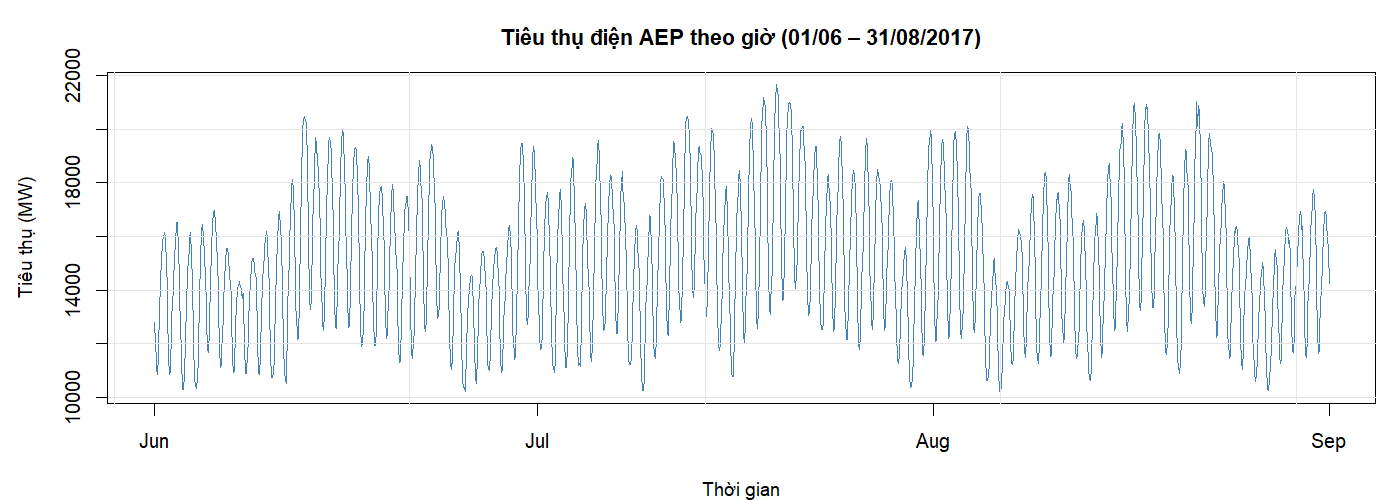
\includegraphics[width=\linewidth]{img/fig_s2_01_full_series.png}
  \caption{Tiêu thụ điện AEP theo giờ, 01/06--31/08/2017}
  \label{fig:full_series}
\end{figure}

\textbf{Chu kỳ ngày và chu kỳ tuần (Hình~\ref{fig:weekly_zoom}).}
Zoom vào 2 tuần đầu cho thấy rõ hai cấu trúc mùa vụ đồng thời:
\begin{itemize}[leftmargin=2em]
  \item \textit{Chu kỳ ngày (24 h)}: tiêu thụ giảm mạnh vào rạng sáng (0--5h),
    phục hồi từ 6h và đạt đỉnh khoảng 9h và 18--20h.
  \item \textit{Chu kỳ tuần}: các ngày cuối tuần (nền hồng) có mức tiêu thụ
    thấp hơn và dạng sóng phẳng hơn so với ngày làm việc.
\end{itemize}

\begin{figure}[H]
  \centering
  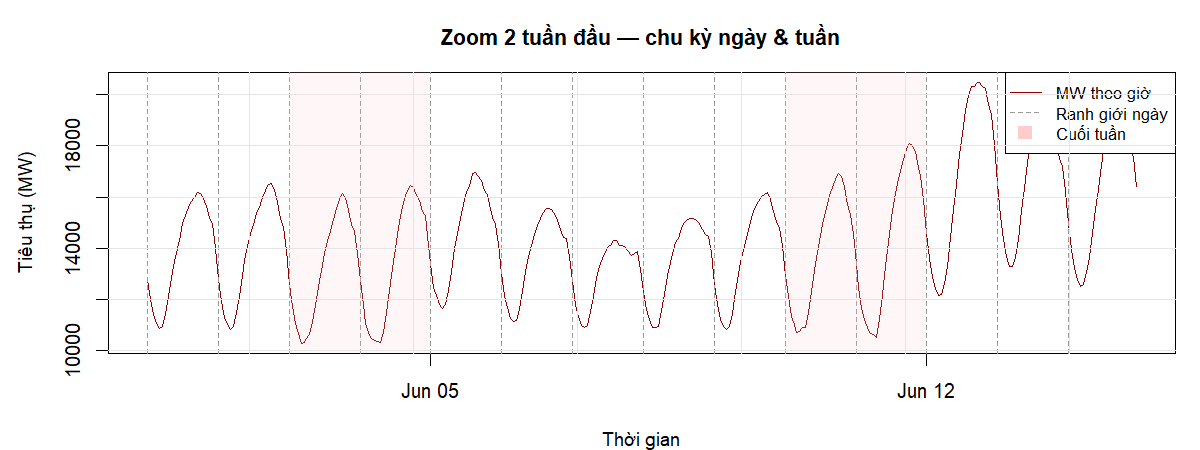
\includegraphics[width=\linewidth]{img/fig_s2_02_weekly_zoom.png}
  \caption{Zoom 2 tuần đầu: chu kỳ ngày và chu kỳ tuần
    (vùng hồng = cuối tuần)}
  \label{fig:weekly_zoom}
\end{figure}

\textbf{Phân bố theo giờ trong ngày (Hình~\ref{fig:diurnal_box}).}
Boxplot cho 24 giờ xác nhận hai đỉnh tiêu thụ rõ rệt: đỉnh sáng ở giờ 9--10 và
đỉnh chiều ở giờ 17--19, với mức thấp nhất vào 3--4 giờ sáng. Phương sai lớn ở
các giờ cao điểm phản ánh sự biến động mạnh giữa ngày thường và cuối tuần.

\begin{figure}[H]
  \centering
  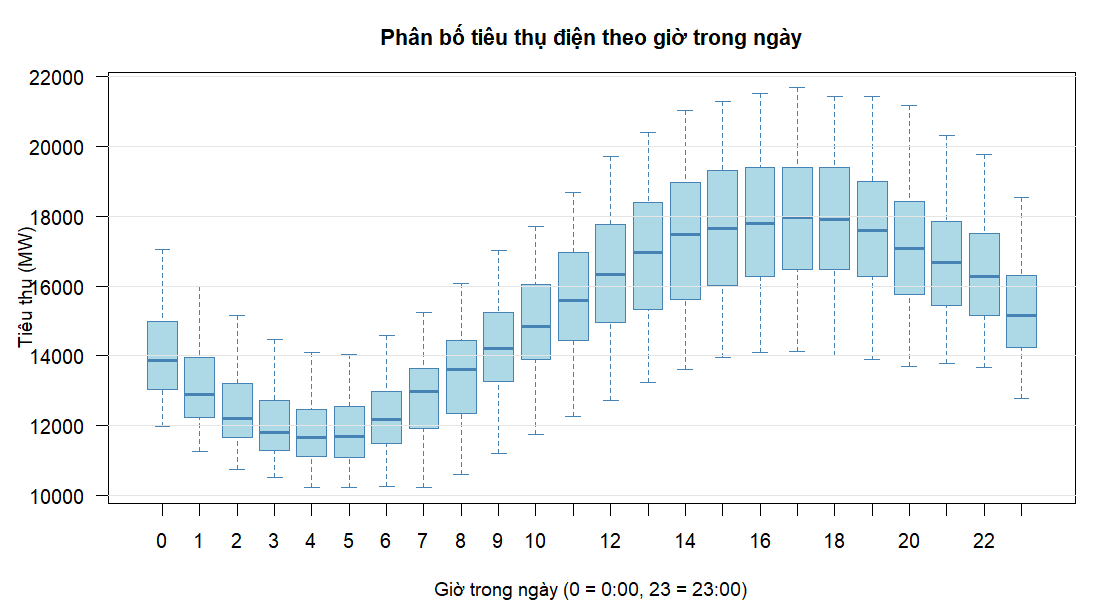
\includegraphics[width=0.9\linewidth]{img/fig_s2_03_diurnal_box.png}
  \caption{Phân bố tiêu thụ điện theo giờ trong ngày (boxplot 24 giờ)}
  \label{fig:diurnal_box}
\end{figure}

\textbf{Ngày thường và cuối tuần (Hình~\ref{fig:weekday_vs_weekend}).}
Profile trung vị theo giờ cho thấy ngày làm việc có mức tiêu thụ cao hơn ổn định
khoảng 1\,000--2\,000 MW với hai đỉnh tương phản rõ ràng. Cuối tuần có đỉnh sáng
xuất hiện muộn hơn (khoảng 10--11h) do sinh hoạt dân dụng chiếm ưu thế.

\begin{figure}[H]
  \centering
  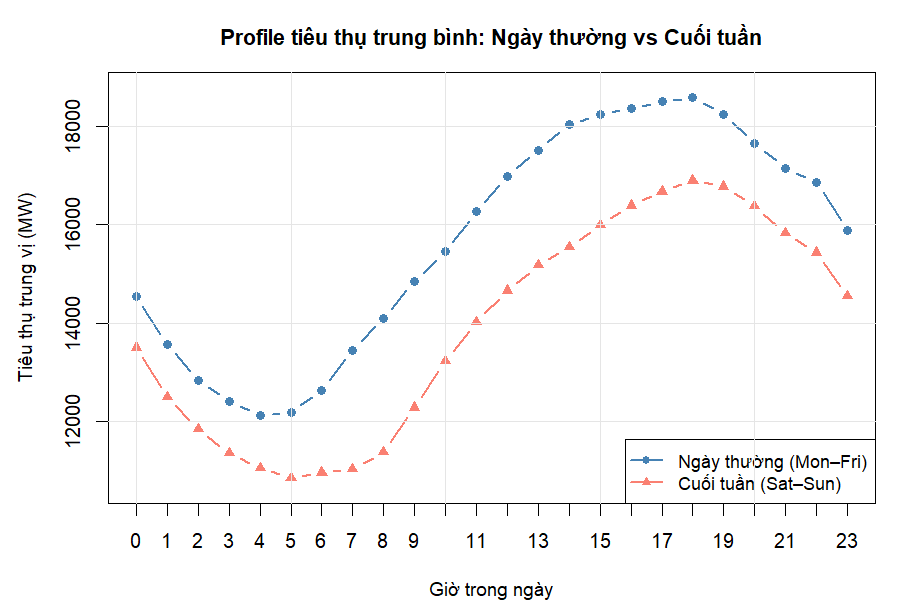
\includegraphics[width=0.82\linewidth]{img/fig_s2_04_weekday_vs_weekend.png}
  \caption{Profile tiêu thụ trung vị: ngày thường (xanh) vs.\ cuối tuần (đỏ)}
  \label{fig:weekday_vs_weekend}
\end{figure}

\textbf{Phân rã cộng tính (Hình~\ref{fig:decompose}).}
Phân rã $Y_t = T_t + S_t + R_t$ với \texttt{frequency = 24} tách chuỗi thành ba
thành phần:
\begin{itemize}[leftmargin=2em]
  \item \textit{Xu hướng ($T_t$)}: dao động nhẹ quanh $\approx 15\,000$ MW,
    không có xu thế đơn điệu.
  \item \textit{Mùa vụ ($S_t$)}: thành phần lặp lại chu kỳ 24 h với biên độ
    khoảng $\pm 3\,000$ MW.
  \item \textit{Phần dư ($R_t$)}: nhiễu còn lại sau khi tách xu hướng và mùa vụ.
\end{itemize}

\begin{figure}[H]
  \centering
  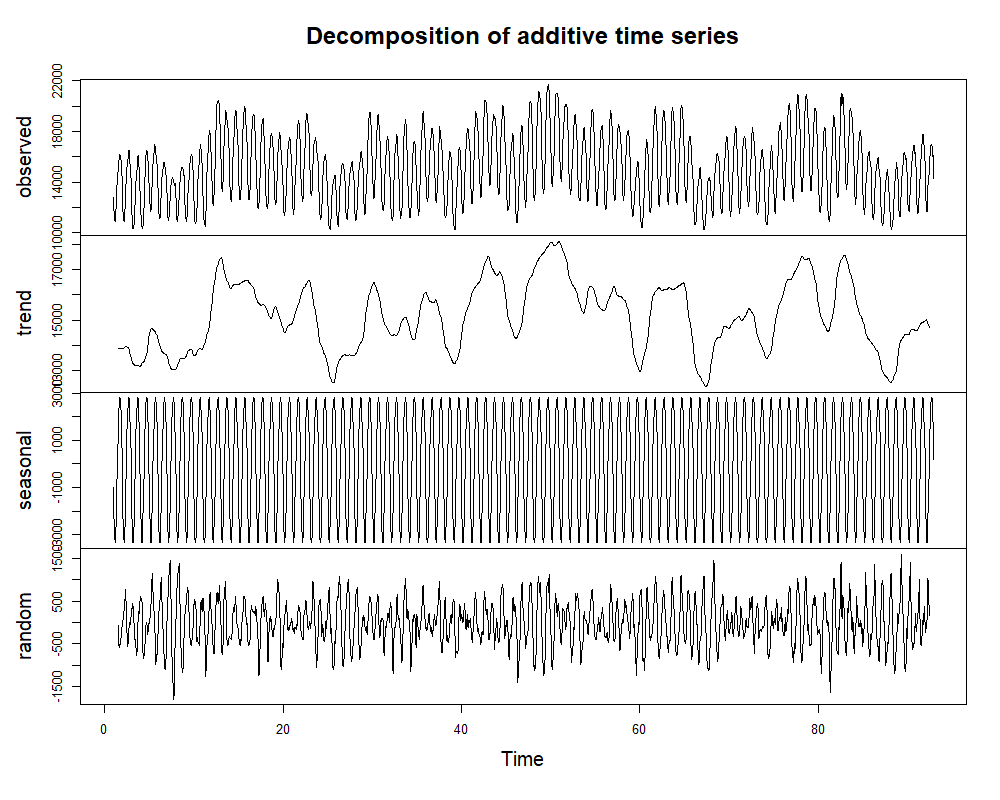
\includegraphics[width=0.92\linewidth]{img/fig_s2_05_decompose.png}
  \caption{Phân rã cộng tính: xu hướng, mùa vụ và phần dư}
  \label{fig:decompose}
\end{figure}

% ============================================================
\subsection{Kiểm định tính dừng: ADF và KPSS}
% ============================================================

Tính dừng là điều kiện nền tảng của các mô hình ARIMA/SARIMA. Nghiên cứu áp dụng
hai kiểm định có \textbf{giả thuyết không đối lập nhau} để bổ trợ lẫn nhau:
\begin{itemize}[leftmargin=2em]
  \item \textbf{ADF} (Augmented Dickey--Fuller): $H_0$: chuỗi \emph{không dừng}
    (có nghiệm đơn vị). $p < 0{,}05 \Rightarrow$ bác bỏ $H_0 \Rightarrow$
    chuỗi dừng.
  \item \textbf{KPSS} (Kwiatkowski--Phillips--Schmidt--Shin): $H_0$: chuỗi
    \emph{dừng}. $p < 0{,}05 \Rightarrow$ bác bỏ $H_0 \Rightarrow$
    chuỗi không dừng.
\end{itemize}

Kết quả được tổng hợp trong Bảng~\ref{tab:stationarity}.

\begin{table}[H]
  \centering
  \caption{Kết quả kiểm định tính dừng}
  \label{tab:stationarity}
  \small
  \begin{tabular}{llccc}
    \toprule
    Kiểm định & Chuỗi & Thống kê & $p$-value & Kết luận \\
    \midrule
    ADF  & Gốc $y_t$             & $-4{,}833$ & $<0{,}01$ & Dừng \\
    KPSS & Gốc $y_t$             & $0{,}459$  & $0{,}052$ & Dừng (biên giới) \\
    ADF  & $\nabla_{24}y_t$ & $-6{,}904$ & $<0{,}01$ & Dừng \\
    \bottomrule
  \end{tabular}
\end{table}

\textbf{Phân tích ACF/PACF (Hình~\ref{fig:acf_pacf}).}
Đồ thị tự tương quan của chuỗi gốc thể hiện các spike lớn có chu kỳ tại lag 24,
48, 72 trong ACF --- đặc trưng của cấu trúc mùa vụ 24 h. PACF cắt cụt sắc nét
sau lag 1--2 với spike phụ tại các bội số của 24, gợi ý thành phần AR bậc thấp
kết hợp với cấu trúc mùa vụ.

\begin{figure}[H]
  \centering
  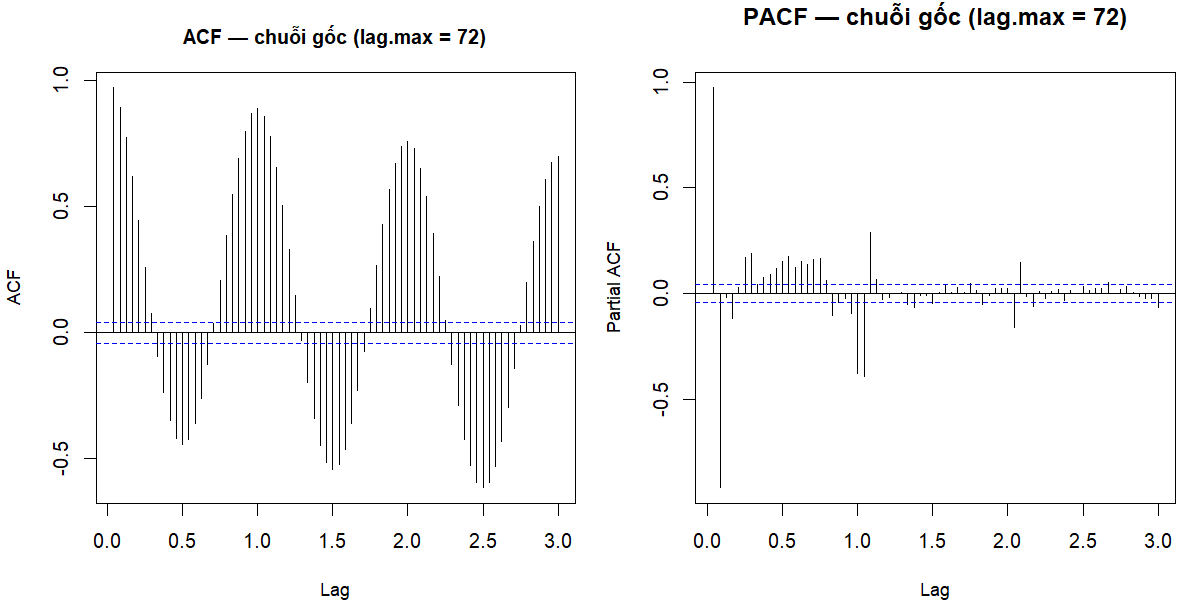
\includegraphics[width=\linewidth]{img/fig_s2_06_acf_pacf.png}
  \caption{ACF và PACF của chuỗi gốc $y_t$ (\texttt{lag.max = 72})}
  \label{fig:acf_pacf}
\end{figure}

\textbf{Chuỗi sau sai phân mùa (Hình~\ref{fig:seasonal_diff}).}
Sau khi áp dụng sai phân mùa $\nabla_{24}y_t = y_t - y_{t-24}$, chuỗi dao động
ổn định quanh 0 và ACF giảm nhanh hơn. Kết quả xác nhận rằng một sai phân mùa
($D = 1$, $s = 24$) là đủ để loại bỏ phần lớn cấu trúc mùa trước khi mô hình
hóa bằng SARIMA.

\begin{figure}[H]
  \centering
  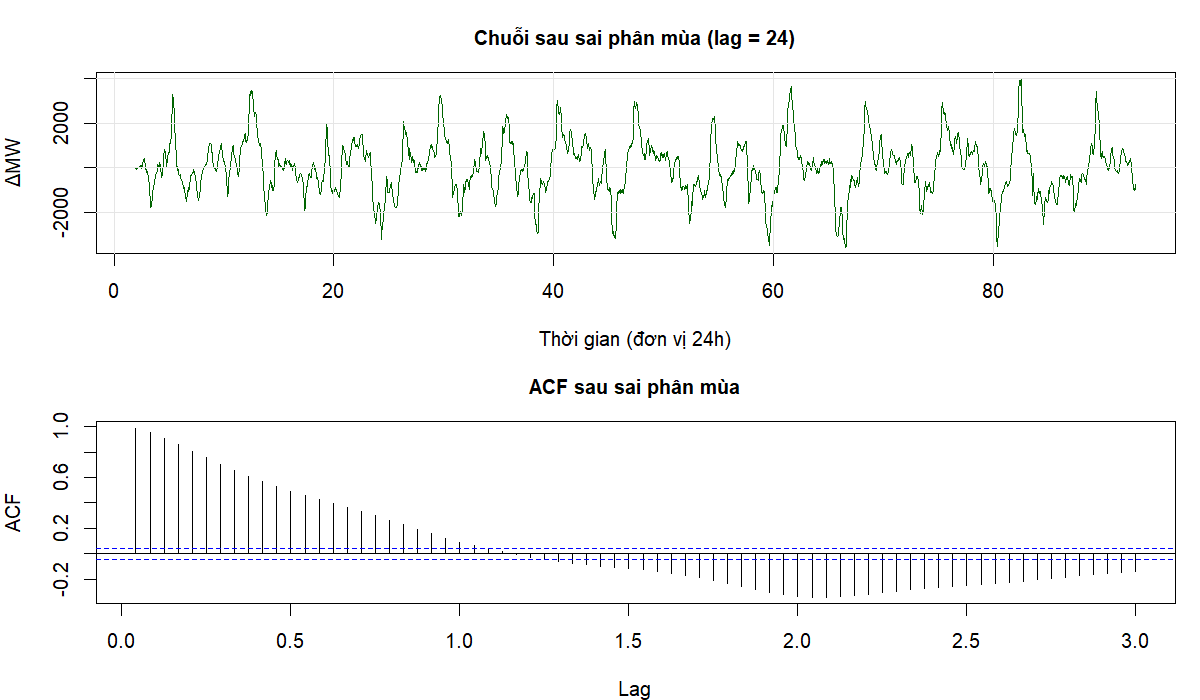
\includegraphics[width=\linewidth]{img/fig_s2_07_seasonal_diff.png}
  \caption{Chuỗi sau sai phân mùa $\nabla_{24}y_t$ và ACF tương ứng}
  \label{fig:seasonal_diff}
\end{figure}

\textbf{Kết luận.}
Cả ADF và KPSS đồng thuận rằng chuỗi gốc $y_t$ là \textbf{dừng về mặt thống kê}
(ADF: $p < 0{,}01$; KPSS: $p = 0{,}052$, biên giới mức 5\%). Tuy nhiên, cấu
trúc mùa vụ mạnh trong ACF cho thấy các mô hình cần xử lý thành phần chu kỳ
24 h một cách tường minh --- đây là lý do chính để đề xuất và so sánh ba phương
pháp M1, M2, M3 trong các phần tiếp theo.

\end{document}